
\documentclass[10pt,a4paper]{article}

%%%%%%%%%%%%%%%%%%%%%%%%%%%%%%%%%%%%%%%%%%%%%%%%%%%%%%%%
%
% Packages and Theorem Environments

\usepackage{graphicx}
\usepackage{psfrag}
\usepackage{epsf}
\usepackage{amsmath,amsfonts,amssymb,latexsym}
\usepackage{enumitem}
\usepackage{algorithmic}
\usepackage{algorithm}
\usepackage[width=160mm,height=240mm,left=25mm,foot=10mm]{geometry}
\usepackage{xcolor}
\usepackage{url}
\usepackage{hyperref}
\usepackage{tikz}



\renewcommand{\theequation}{\thesection.\arabic{equation}}
\newcommand{\makeTiny}[1]{{\tiny #1}}
\newcommand{\work}{\tiny}
\newcommand{\ignore}[1]{}
\newcommand{\startClaims}{\setcounter{claim}{0}}
\newtheorem{theorem}{Theorem}[section]
\newtheorem{corollary}[theorem]{Corollary}
\newtheorem{lemma}[theorem]{Lemma}
\newtheorem{proposition}[theorem]{Proposition}
\newtheorem{conjecture}[theorem]{Conjecture}
\newtheorem{problem}[theorem]{Problem}
\newtheorem{question}[theorem]{Question}
\newtheorem{definition}[theorem]{Definition}
\newtheorem{task}[theorem]{Task}
\newtheorem{claim}{Claim}
\newtheorem{remark}[theorem]{Remark}
\newtheorem{observation}[theorem]{Observation}





\title{MATH 351--004 -- Assignment \#$1$\\
}

\author{Alex Iacob\\
ai9388}

\date{September 2, 2021}


%%%%%%%%%%%%%%%%%%%%%%%%%%%%%%%%%%%%%%%%%%%%%%%%%%%%%%%%
%
% Author's definitions


\newcommand{\NN}{\mathbb N}
\newcommand{\ZZ}{\mathbb Z}
\newcommand{\QQ}{\mathbb Q}
\newcommand{\RR}{\mathbb R}

\newcommand{\BB}{\mathcal B}
\newcommand{\ZT}{\mathcal Z}

\newcommand{\Cl}{\operatorname{Cl}}
\newcommand{\Bd}{\operatorname{Bd}}
\newcommand{\row}{\operatorname{row}}
\newcommand{\col}{\operatorname{col}}
\newcommand{\Span}{\operatorname{span}}
\newcommand{\convhull}{\operatorname{conv.hull}}
\newcommand{\tr}{\operatorname{tr}}

\newcommand{\diam}{\operatorname{diam}}

\DeclareUnicodeCharacter{2212}{-}
\graphicspath{hw1}

\begin{document}

\maketitle

\begin{center}
{\bf \large Part 2}
\end{center}

\subsection*{Problem 1.8
Let S be a finite set of 3-letter and/or 4-letter words. In this case, the word graph $G(S)$ of $S$ is
that graph whose vertex set is S and such that two vertices (words) $w_{1}$ and $w_{2}$ are adjacent if either (1) or (2) below occurs:\\
(1) one of the words can be obtained from the other by replacing one letter by another letter,\\
(2) $w_{1}$ is a 3-letter word and $w_{2}$ is a 4-letter word and $w_{2}$ can be obtained from $w_{1}$ by the
insertion of a single letter (anywhere, including the beginning or the end) into $w_{1}$.\\
}

\subsection*{
(a) Find six sets $S_{1}$, $S_{2}$, …, $S_{6}$ of 3-letter and/or 4-letter words so that for each integer i $(1 <= i <=6)$ the graph $G_{i}$ of Figure 1.13 is the word graph of $S_{i}$.\\
(b) For another graph $H$ (of your choice), determine whether $H$ is a word graph of some set.\\
}
(a)\\
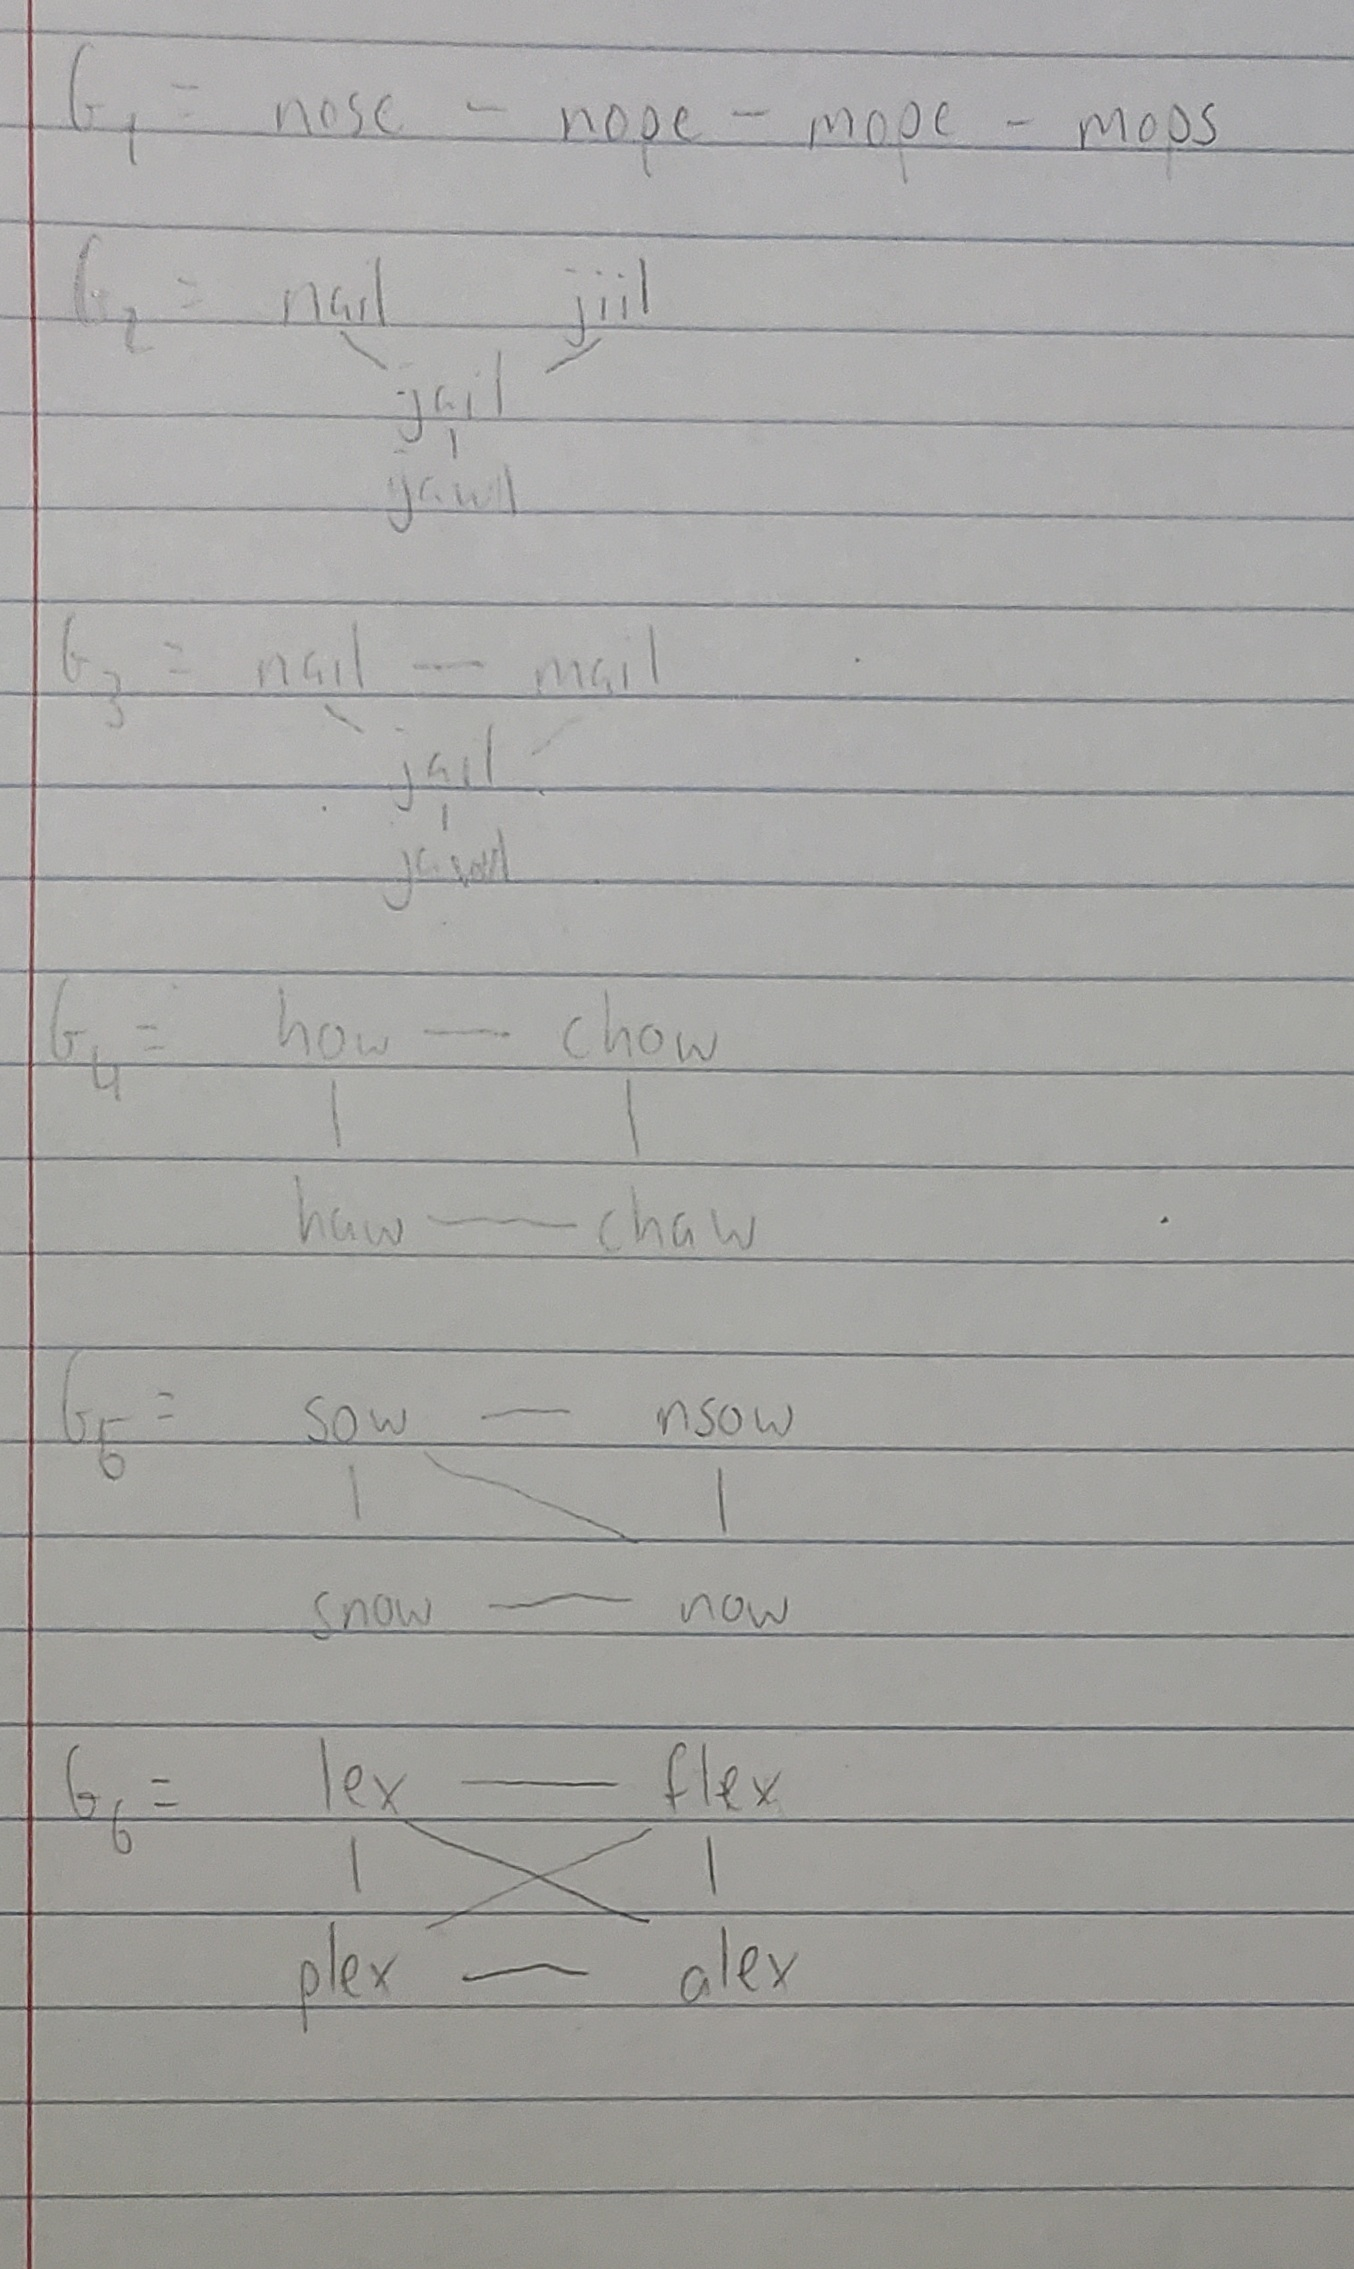
\includegraphics[width=7cm]{question1.8a}

(b)\\
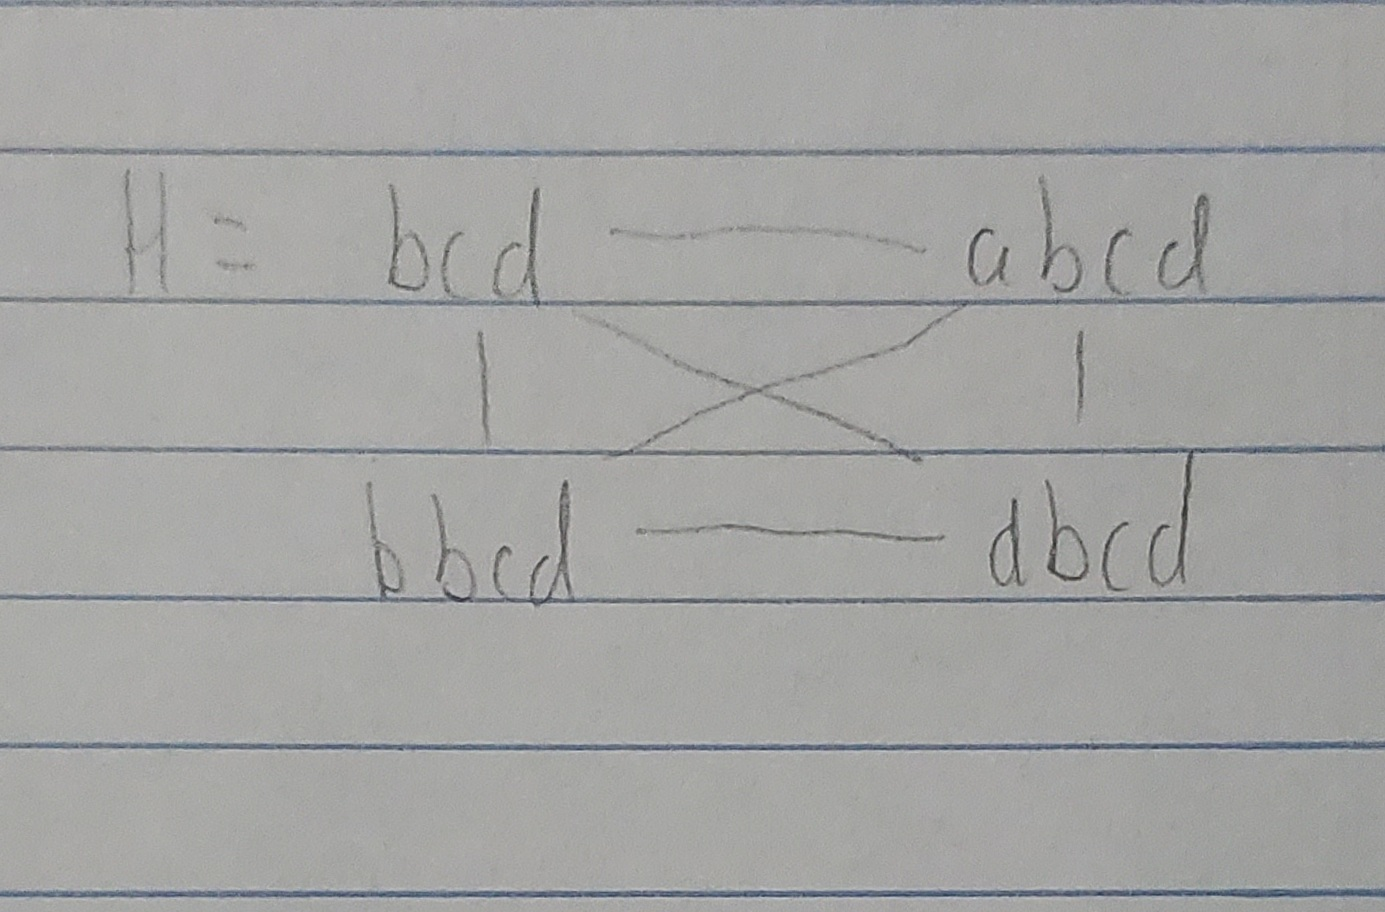
\includegraphics[width=7cm]{question1.8b}

\subsection*{Problem 1.16
Let $P = (u = v_{0}, v_{1}, ..., v_{k} = v)$, $k >= 1$, be a $u - v$ geodesic in a connected graph $G$. 
Prove that $d(u, v_{i}) = i$ for each integer $i$ with $1 <= i <= k$.
}

In order for a graph to be connected, there is a path from any point to any other point on the graph.
Because of this connectivity, the shortest path between two points must be $1$. The largest path between any 
two points is the amount of nodes, $k$. Anything in between these two values is the path length from any two points.

\subsection*{Problem 1.19
Theorem 1.10 states that a graph $G$ of order 3 or more is connected if and only if $G$ contains
two distinct vertices $u$ and $v$ such that $G − u$ and $G − v$ are connected. Based on this, one might
suspect that the following statement is true. Every connected graph $G$ of order 4 or more
contains three distinct vertices $u$, $v$ and $w$ such that $G$ − $u$, $G$ − $v$ and $G$ − $w$ are connected. Is it$?$
}

This is not true. Adding a third distinct vertex does not further prove that the given graph is connected, rather the opposite.

\subsection*{Problem 1.20
(a)Let $u$ and $v$ be distinct vertices in a connected graph $G$. There may be several connected
subgraphs of $G$ containing $u$ and $v$. What is the minimum size of a connected subgraph of $G$
containing $u$ and $v$? Explain your answer.\\
(b)Does the question in (a) suggest another question to you?
}

(a) Both subgraphs can be single vertices, so the minimum size of a connected subgraph is 1.\\
(b) The suggested question is "What is the minimum possible size for a connected subgraph?"


\end{document} 




















